%%===================================================================
%% Lecture 18 -- Electroweak Gauge-Boson Masses, Lepton Masses,
%%               and Higgs Couplings in the Lepton Standard Model
%% 77609 -- Introduction to Elementary Particles
%% Date: 14/06/2026
%% Lecturer: Prof. Yonit Hochberg
%%===================================================================

\section{Lecture 18 -- Electroweak Gauge-Boson Masses, Lepton Masses, and Higgs Couplings}\label{sec:lec18}
\begin{center}
\begin{tabular}{ll}
  \textbf{Date:}\quad 14/06/2026 & \\
\end{tabular}
\end{center}
\hrule\vspace{1.5em}

%%------------------------------------------------------------------
\subsection{Overview}\label{subsec:lec18:overview}

Lecture~17 constructed the Lepton Standard Model (LSM): a local
$SU(2)_L\times U(1)_Y$ gauge theory with a scalar doublet
$\phi=(\phi^+,\phi^0)^T$ and lepton fields
$L_{Li}=(\nu_{Li},e_{Li})^T$, $E_{Ri}$. The Higgs vacuum
$\langle\phi\rangle=(0,v)^T/\sqrt2$ preserves exactly one generator,
$Q=T^3+Y$, so the symmetry breaking pattern is
$SU(2)_L\times U(1)_Y\to U(1)_{\rm EM}$.

Today we finish extracting the physical content of this theory. The four gauge
fields of the symmetric theory, $W^1_\mu,W^2_\mu,W^3_\mu,B_\mu$, are not all
mass eigenstates. The charged combinations become $W^\pm_\mu$, and the neutral
fields $W^3_\mu,B_\mu$ rotate by the weak mixing angle into the massive
$Z_\mu$ and the massless photon $A_\mu$. The same vacuum expectation value
also turns the charged-lepton Yukawa couplings into Dirac masses, while the
neutrinos remain massless in this minimal lepton theory.

The last part of the lecture organizes the interaction terms in the mass basis.
This is the basis used in experiments: particles have definite mass and
definite electromagnetic charge. In this basis we can read off the Higgs
self-couplings, the Higgs couplings to $W$ and $Z$ bosons, and the Higgs
couplings to charged leptons. The essential structural lesson is that many
apparently independent measured quantities are related because they all descend
from the same gauge symmetry and the same Higgs vev.

%%==================================================================
\subsection{Charged and Neutral Gauge-Boson Mass Eigenstates}\label{subsec:lec18:gauge-mass-eigenstates}

\subsubsection*{Mathematical Setup}

At the end of Lecture~17 the gauge-boson mass terms came from the scalar
kinetic term evaluated on the vacuum:
\begin{equation}
  \Lag_{\rm mass}
  =\frac{v^2}{8}\Big[g^2\big(W^1_\mu W^{1\mu}+W^2_\mu W^{2\mu}\big)
  +\big(gW^3_\mu-g'B_\mu\big)\big(gW^{3\mu}-g'B^\mu\big)\Big] .
  \label{eq:lec18:starting-mass-terms}
\end{equation}
Here $g$ is the $SU(2)_L$ gauge coupling, $g'$ is the $U(1)_Y$ gauge coupling,
$v$ is the Higgs vev, and $B_\mu$ is the hypercharge gauge boson. The charged
sector $W^1,W^2$ is already diagonal after forming complex combinations; the
neutral sector $W^3,B$ still has mixing.

\dfn[dfn:lec18:weinberg-angle]{Weak Mixing Angle}{
The weak mixing angle, also called the Weinberg angle, is defined by
\begin{equation}
  \boxed{\;\tan\theta_W=\frac{g'}{g}\;} .
  \label{eq:lec18:weinberg-angle}
\end{equation}
Equivalently,
\begin{equation*}
  \sin\theta_W=\frac{g'}{\sqrt{g^2+g'^2}},
  \qquad
  \cos\theta_W=\frac{g}{\sqrt{g^2+g'^2}} .
\end{equation*}
}

\textit{Significance:} $\theta_W$ is the rotation angle between the neutral interaction basis $(W^3,B)$ and the neutral mass basis $(Z,A)$.

Define the charged fields by
\begin{equation}
  \boxed{\;W^\pm_\mu=\frac{1}{\sqrt2}\big(W^1_\mu\mp iW^2_\mu\big)\;}
  \label{eq:lec18:wpm-definition}
\end{equation}
and the neutral fields by the orthogonal rotation
\begin{equation}
  \boxed{\;
  \begin{pmatrix} Z_\mu \\ A_\mu \end{pmatrix}
  =
  \begin{pmatrix}
    \cos\theta_W & -\sin\theta_W \\
    \sin\theta_W & \phantom{-}\cos\theta_W
  \end{pmatrix}
  \begin{pmatrix} W^3_\mu \\ B_\mu \end{pmatrix} .\;}
  \label{eq:lec18:neutral-rotation}
\end{equation}

\textit{Significance:} $W^\pm_\mu$ carry electromagnetic charge $\pm1$, while $A_\mu$ and $Z_\mu$ are electrically neutral; $A_\mu$ is the gauge boson of the unbroken $U(1)_{\rm EM}$.

To see the diagonalization explicitly, invert Eq.~\eqref{eq:lec18:neutral-rotation}:
\begin{equation}
  W^3_\mu=\cos\theta_W Z_\mu+\sin\theta_W A_\mu,
  \qquad
  B_\mu=-\sin\theta_W Z_\mu+\cos\theta_W A_\mu .
  \label{eq:lec18:neutral-inverse}
\end{equation}
Then the neutral mass combination becomes
\begin{align}
  gW^3_\mu-g'B_\mu
  &=g(\cos\theta_W Z_\mu+\sin\theta_W A_\mu)
    -g'(-\sin\theta_W Z_\mu+\cos\theta_W A_\mu) \notag\\
  &=(g\cos\theta_W+g'\sin\theta_W)Z_\mu
    +(g\sin\theta_W-g'\cos\theta_W)A_\mu .
  \label{eq:lec18:neutral-combination-expanded}
\end{align}
Using $\tan\theta_W=g'/g$, the photon coefficient vanishes:
\begin{equation}
  g\sin\theta_W-g'\cos\theta_W=0,
  \label{eq:lec18:photon-coefficient-vanishes}
\end{equation}
while
\begin{equation}
  g\cos\theta_W+g'\sin\theta_W=\sqrt{g^2+g'^2} .
  \label{eq:lec18:z-coefficient}
\end{equation}
Substituting into Eq.~\eqref{eq:lec18:starting-mass-terms} gives the diagonal
mass Lagrangian
\begin{equation}
  \boxed{\;
  \Lag_{\rm mass}
  =\frac{g^2v^2}{4}\,W^+_\mu W^{-\mu}
   +\frac{(g^2+g'^2)v^2}{8}\,Z_\mu Z^\mu
   +0\cdot A_\mu A^\mu .\;}
  \label{eq:lec18:diagonal-mass-lagrangian}
\end{equation}

\textit{Significance:} The photon is massless because it is attached to the unbroken generator $Q$, whereas the three gauge bosons associated with broken directions acquire mass.

\begin{figure}[ht]
\centering
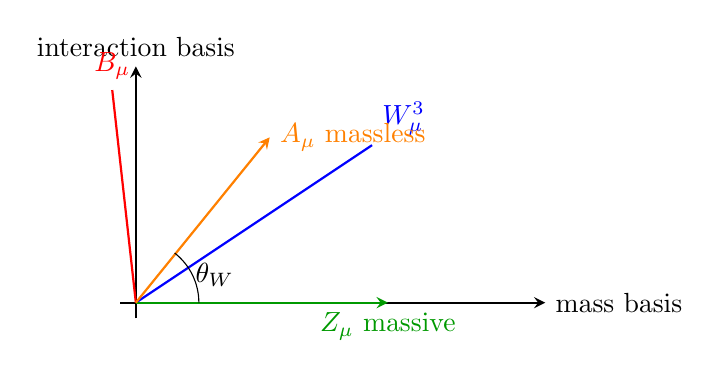
\begin{tikzpicture}[>=stealth,scale=1.0]
  \draw[->,thick] (-0.2,0) -- (5.2,0) node[right] {mass basis};
  \draw[->,thick] (0,-0.2) -- (0,3.0) node[above] {interaction basis};
  \draw[thick,blue] (0,0) -- (3.0,2.0) node[above right] {$W^3_\mu$};
  \draw[thick,red] (0,0) -- (-0.3,2.7) node[above] {$B_\mu$};
  \draw[thick,green!60!black,->] (0,0) -- (3.2,0) node[below] {$Z_\mu$ massive};
  \draw[thick,orange,->] (0,0) -- (1.7,2.1) node[right] {$A_\mu$ massless};
  \draw (0.8,0) arc[start angle=0,end angle=52,radius=0.8];
  \node at (1.0,0.35) {$\theta_W$};
\end{tikzpicture}
\caption{The neutral electroweak fields rotate from the interaction basis $(W^3_\mu,B_\mu)$ to the mass basis $(Z_\mu,A_\mu)$. The direction orthogonal to the Higgs mass term is the photon.}
\label{fig:lec18:weak-mixing}
\end{figure}

\nt{Pitfall: $W^+_\mu$ and $W^-_\mu$ are complex conjugate charged fields, so their mass term is $m_W^2W^+_\mu W^{-\mu}$ with no factor of $1/2$. The $Z_\mu$ is a real neutral vector, so its mass term is $\tfrac12m_Z^2Z_\mu Z^\mu$. Mixing these normalizations changes $m_Z$ by a false factor of $\sqrt2$.}

\subsubsection*{Method}

To extract electroweak vector masses from $|D_\mu\phi|^2$:
\begin{enumerate}
  \item Put the Higgs doublet in unitary gauge and keep only its vev, $\langle\phi\rangle=(0,v)^T/\sqrt2$.
  \item Compute $D_\mu\langle\phi\rangle$ and form $(D_\mu\langle\phi\rangle)^\dagger D^\mu\langle\phi\rangle$.
  \item Identify charged combinations $W^\pm=(W^1\mp iW^2)/\sqrt2$.
  \item Write the neutral quadratic form in the $(W^3,B)$ basis.
  \item Rotate by $\theta_W$ so that one combination appears in the mass term ($Z$) and the orthogonal combination does not ($A$).
  \item Compare with $m_W^2W^+W^-$ and $\tfrac12m_Z^2Z^2$ to read off masses.
\end{enumerate}

\ex[ex:lec18:neutral-diagonalization]{Worked Example: Finding the Photon Direction}{
Start from the neutral mass term
\begin{equation*}
  \Lag_{\rm neutral}=\frac{v^2}{8}(gW^3_\mu-g'B_\mu)^2 .
\end{equation*}
The massive direction is the vector $(g,-g')$ in the $(W^3,B)$ plane. A massless direction must be orthogonal to it:
\begin{equation*}
  (g,-g')\cdot(a,b)=ga-g'b=0
  \quad\Longrightarrow\quad
  \frac{a}{b}=\frac{g'}{g} .
\end{equation*}
Normalize the vector $(g',g)$:
\begin{equation*}
  A_\mu=\frac{g'}{\sqrt{g^2+g'^2}}W^3_\mu
       +\frac{g}{\sqrt{g^2+g'^2}}B_\mu
       =\sin\theta_W W^3_\mu+\cos\theta_W B_\mu .
\end{equation*}
The orthogonal normalized direction is
\begin{equation*}
  Z_\mu=\cos\theta_W W^3_\mu-\sin\theta_W B_\mu .
\end{equation*}
Thus the massless eigenstate is the photon and the massive neutral eigenstate is the $Z$ boson.
}

%%==================================================================
\subsection{Vector-Boson Masses and the \texorpdfstring{$\rho$}{rho} Parameter}\label{subsec:lec18:rho-parameter}

\subsubsection*{Physical Motivation}

Spontaneous symmetry breaking is not merely a mechanism for producing masses.
Because the masses come from one Higgs vev and a gauge-invariant kinetic term,
they satisfy relations. These relations compare quantities that experiments
measure in different ways: masses from the spectrum, and couplings from
interaction rates. Agreement is therefore a nontrivial test of the electroweak
symmetry-breaking sector.

Reading masses from Eq.~\eqref{eq:lec18:diagonal-mass-lagrangian} gives
\begin{equation}
  \boxed{\;m_W^2=\frac{g^2v^2}{4},
  \qquad
  m_Z^2=\frac{(g^2+g'^2)v^2}{4},
  \qquad
  m_A^2=0 .\;}
  \label{eq:lec18:gauge-boson-masses}
\end{equation}

\textit{Significance:} Electroweak symmetry breaking predicts exactly three massive weak bosons and one massless photon, matching the unbroken $U(1)_{\rm EM}$.

Taking the ratio,
\begin{equation}
  \frac{m_W^2}{m_Z^2}
  =\frac{g^2}{g^2+g'^2}
  =\cos^2\theta_W .
  \label{eq:lec18:mw-mz-ratio}
\end{equation}
This motivates the definition
\begin{equation}
  \boxed{\;\rho\equiv\frac{m_W^2}{m_Z^2\cos^2\theta_W}\;} .
  \label{eq:lec18:rho-definition}
\end{equation}

\textit{Significance:} $\rho$ packages the mass--coupling relation into one observable number; in the minimal Higgs-doublet theory, $\rho=1$ at tree level.

Substituting Eq.~\eqref{eq:lec18:mw-mz-ratio} immediately gives
\begin{equation}
  \boxed{\;\rho_{\rm LSM}=1\quad\text{(tree level, one }SU(2)_L\text{ Higgs doublet).}\;}
  \label{eq:lec18:rho-one}
\end{equation}

\textit{Significance:} The measured near-unity of $\rho$ is evidence that electroweak symmetry breaking is dominantly caused by scalar doublet vevs rather than arbitrary scalar representations.

The lecture quoted the experimental masses
\begin{equation}
  m_W=80.385\pm0.015\ \mathrm{GeV},
  \qquad
  m_Z=91.1876\pm0.0021\ \mathrm{GeV} .
  \label{eq:lec18:measured-wz-masses}
\end{equation}
Assuming $\rho=1$, these determine
\begin{equation}
  \boxed{\;\sin^2\theta_W=1-\frac{m_W^2}{m_Z^2}
  \simeq0.2229\pm0.0004 .\;}
  \label{eq:lec18:sin2-from-masses}
\end{equation}

\textit{Significance:} The same $\sin^2\theta_W$ can be extracted from interaction rates; consistency between the two determinations tests the whole electroweak construction.

\ex[ex:lec18:rho-calculation]{Worked Example: Testing the Tree-Level Mass Relation}{
Suppose an experiment measures $m_W$, $m_Z$, and an interaction observable that gives $\sin^2\theta_W$. To test the Higgs-doublet prediction:
\begin{enumerate}
  \item Convert the measured angle to $\cos^2\theta_W=1-\sin^2\theta_W$.
  \item Form
  \begin{equation*}
    \rho=\frac{m_W^2}{m_Z^2\cos^2\theta_W} .
  \end{equation*}
  \item If the minimal tree-level LSM is correct up to small loop corrections, the answer should be close to $1$.
\end{enumerate}
For example, if the mass ratio itself is used to infer the angle,
\begin{equation*}
  \cos^2\theta_W=\frac{m_W^2}{m_Z^2}
  \quad\Longrightarrow\quad
  \rho=\frac{m_W^2}{m_Z^2(m_W^2/m_Z^2)}=1 .
\end{equation*}
The real test is that an independently measured weak mixing angle agrees with this mass prediction.
}

\nt{Pitfall: $\rho=1$ is not a definition of $\theta_W$ in all contexts. The clean test is to compare the mass ratio with an independently measured weak mixing angle from neutral-current or electromagnetic interaction data.}

%%==================================================================
\subsection{The Covariant Derivative in the Mass Basis}\label{subsec:lec18:covariant-derivative-mass-basis}

\subsubsection*{Conceptual Background}

Before symmetry breaking, $W^a_\mu$ and $B_\mu$ are the natural fields because
they transform simply under $SU(2)_L\times U(1)_Y$. After symmetry breaking,
experiments see $W^\pm_\mu$, $Z_\mu$, and $A_\mu$. We therefore rewrite the
same covariant derivative in the mass basis.

With the convention
\begin{equation}
  T^\pm=\frac{1}{\sqrt2}\big(T^1\pm iT^2\big),
  \label{eq:lec18:tpm-definition}
\end{equation}
the $SU(2)$ charged part obeys
\begin{equation}
  W^1_\mu T^1+W^2_\mu T^2=W^+_\mu T^+ + W^-_\mu T^- .
  \label{eq:lec18:charged-generator-identity}
\end{equation}
Using Eq.~\eqref{eq:lec18:neutral-inverse}, the full covariant derivative becomes
\begin{equation}
  \boxed{\;
  D_\mu=\partial_\mu
  +ig\big(W^+_\mu T^+ + W^-_\mu T^-\big)
  +ieA_\mu Q
  +i\frac{g}{\cos\theta_W}Z_\mu\big(T^3-\sin^2\theta_W Q\big)\;}
  \label{eq:lec18:covariant-derivative-mass-basis}
\end{equation}
where
\begin{equation}
  \boxed{\;e=g\sin\theta_W=g'\cos\theta_W,
  \qquad Q=T^3+Y .\;}
  \label{eq:lec18:e-charge-relation}
\end{equation}

\textit{Significance:} The photon couples universally to electric charge $Q$ with coupling $e$, while the $Z$ couples to the shifted weak-isospin charge $T^3-\sin^2\theta_W Q$.

\subsubsection*{Method}

To find the gauge couplings of a specific field:
\begin{enumerate}
  \item Identify whether the field is an $SU(2)_L$ doublet or singlet.
  \item Insert its $T^3$ eigenvalue and hypercharge $Y$.
  \item Compute $Q=T^3+Y$.
  \item The coefficient of $A_\mu$ is $ieQ$.
  \item The coefficient of $Z_\mu$ is $i(g/\cos\theta_W)(T^3-\sin^2\theta_W Q)$.
  \item The charged-current $W^\pm$ couplings are present only when $T^\pm$ connects two components of an $SU(2)_L$ doublet.
\end{enumerate}

\nt{Pitfall: $T^3=0$ for $SU(2)_L$ singlets. Therefore $e_R$, $\mu_R$, and $\tau_R$ have $Q=Y=-1$ and no charged-current $W^\pm$ coupling.}

%%==================================================================
\subsection{Charged-Lepton Masses and Massless Neutrinos}\label{subsec:lec18:lepton-masses}

\subsubsection*{Physical Motivation}

In the symmetric theory the charged leptons are chiral: the left-handed fields
belong to $SU(2)_L$ doublets, while the right-handed fields are singlets. A
bare Dirac mass would not be gauge invariant. The Higgs vev solves this by
turning the gauge-invariant Yukawa interaction into a mass term after symmetry
breaking.

In the charged-lepton mass basis, the three left-handed doublets and three
right-handed singlets are written as
\begin{equation}
  L_{L1}=\begin{pmatrix}\nu_{eL}\\ e_L\end{pmatrix},
  \qquad
  L_{L2}=\begin{pmatrix}\nu_{\mu L}\\ \mu_L\end{pmatrix},
  \qquad
  L_{L3}=\begin{pmatrix}\nu_{\tau L}\\ \tau_L\end{pmatrix},
  \label{eq:lec18:left-lepton-doublets}
\end{equation}
with right-handed singlets
\begin{equation}
  E_{R1}=e_R,
  \qquad
  E_{R2}=\mu_R,
  \qquad
  E_{R3}=\tau_R .
  \label{eq:lec18:right-lepton-singlets}
\end{equation}
The Yukawa matrix has been diagonalized and made real:
\begin{equation}
  Y^e=\operatorname{diag}(y_e,y_\mu,y_\tau),
  \qquad
  y_e<y_\mu<y_\tau .
  \label{eq:lec18:diagonal-yukawa}
\end{equation}

In unitary gauge,
\begin{equation}
  \phi=\frac{1}{\sqrt2}\begin{pmatrix}0\\ v+h\end{pmatrix} .
  \label{eq:lec18:unitary-doublet-again}
\end{equation}
Substituting this into
$\Lag_{\rm Yuk}=-Y^e_{ij}\bar L_{Li}\phi E_{Rj}+\mathrm{h.c.}$ gives
\begin{equation}
  \Lag_{\rm Yuk}
  =-\sum_{\ell=e,\mu,\tau}\frac{y_\ell v}{\sqrt2}\,\bar\ell_L\ell_R
   -\sum_{\ell=e,\mu,\tau}\frac{y_\ell}{\sqrt2}\,h\bar\ell_L\ell_R
   +\mathrm{h.c.}
  \label{eq:lec18:yukawa-expanded}
\end{equation}
Therefore
\begin{equation}
  \boxed{\;m_e=\frac{y_ev}{\sqrt2},
  \qquad
  m_\mu=\frac{y_\mu v}{\sqrt2},
  \qquad
  m_\tau=\frac{y_\tau v}{\sqrt2}.\;}
  \label{eq:lec18:charged-lepton-masses}
\end{equation}

\textit{Significance:} Charged-lepton masses are not independent of Higgs interactions; the same Yukawa coupling fixes both $m_\ell$ and the $h\bar\ell\ell$ vertex.

The measured charged-lepton masses quoted in the lecture are
\begin{equation}
  m_e=0.510998928\ \mathrm{MeV},
  \qquad
  m_\mu=105.6583715\ \mathrm{MeV},
  \qquad
  m_\tau=1776.82\ \mathrm{MeV} .
  \label{eq:lec18:measured-lepton-masses}
\end{equation}
In contrast, the minimal LSM contains no right-handed neutrino field and no
renormalizable neutrino mass term. Thus
\begin{equation}
  \boxed{\;m_{\nu_e}=m_{\nu_\mu}=m_{\nu_\tau}=0\quad\text{in the minimal LSM}.\;}
  \label{eq:lec18:neutrinos-massless}
\end{equation}

\textit{Significance:} Neutrino masses observed in nature require physics beyond this minimal lepton model, such as right-handed neutrinos or higher-dimensional operators.

\ex[ex:lec18:higgs-lepton-coupling]{Worked Example: Which Charged Lepton Couples Most Strongly to the Higgs?}{
The Higgs--lepton interaction from Eq.~\eqref{eq:lec18:yukawa-expanded} is
\begin{equation*}
  \Lag_{h\ell\ell}=-\sum_{\ell=e,\mu,\tau}\frac{m_\ell}{v}\,h\bar\ell\ell .
\end{equation*}
Thus the coupling strength is proportional to $m_\ell/v$. Since
\begin{equation*}
  m_\tau>m_\mu>m_e,
\end{equation*}
the hierarchy of Higgs couplings is
\begin{equation*}
  g_{h\tau\tau}>g_{h\mu\mu}>g_{hee} .
\end{equation*}
The Higgs couples most strongly to the $\tau$ among the charged leptons. It has no tree-level neutrino Yukawa coupling in the minimal LSM because there is no corresponding neutrino mass term.
}

\nt{Pitfall: the fermion mass term has the form $-m\bar\ell_L\ell_R+\mathrm{h.c.}$, not $-\tfrac12m^2\ell^2$. Fermion masses have dimension one and appear linearly in the Lagrangian coefficient.}

%%==================================================================
\subsection{Interactions in the Mass Basis}\label{subsec:lec18:mass-basis-interactions}

\subsubsection*{Physical Motivation}

After finding the spectrum, the next question is: how do the physical particles
interact? In the mass basis the answer separates into several recognizable
classes: Higgs self-interactions, Higgs--gauge interactions, Higgs--lepton
interactions, QED interactions, neutral-current weak interactions, and
charged-current weak interactions. The lecture began this organization and
worked out the Higgs-related terms explicitly.

The Higgs part of the Lagrangian in the mass basis is
\begin{equation}
  \boxed{\;
  \begin{aligned}
  \Lag_h={}&\frac12\partial_\mu h\partial^\mu h
  -\frac12m_h^2h^2
  -\frac{m_h^2}{2v}h^3
  -\frac{m_h^2}{8v^2}h^4 \\
  &+m_W^2W^-_\mu W^{+\mu}\left(\frac{2h}{v}+\frac{h^2}{v^2}\right)
  +\frac12m_Z^2Z_\mu Z^\mu\left(\frac{2h}{v}+\frac{h^2}{v^2}\right) \\
  &-\frac{h}{v}\left(m_e\bar e_Le_R+m_\mu\bar\mu_L\mu_R+m_\tau\bar\tau_L\tau_R+\mathrm{h.c.}\right) .
  \end{aligned}\;}
  \label{eq:lec18:higgs-interaction-lagrangian}
\end{equation}

\textit{Significance:} Every Higgs coupling in this expression is fixed by measured masses and the single scale $v$; the Higgs couples more strongly to heavier particles.

\begin{figure}[ht]
\centering
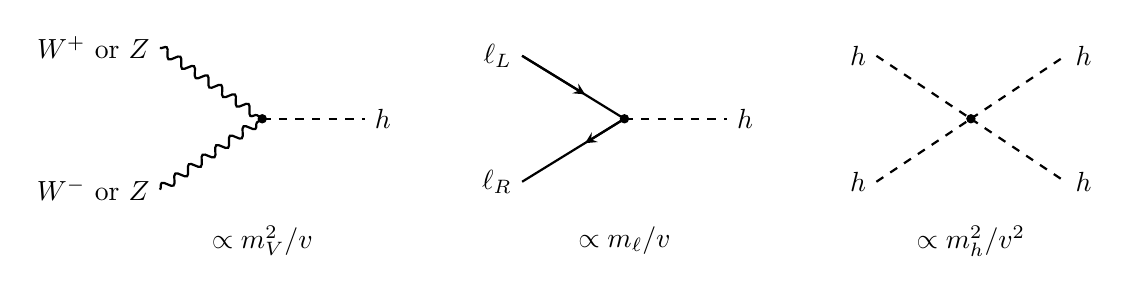
\begin{tikzpicture}[>=stealth,scale=1.0]
  \begin{scope}[xshift=-4.6cm]
    \coordinate (c) at (0,0);
    \draw[decorate,decoration={snake,amplitude=1.6pt,segment length=6pt},thick]
      (-1.3,0.9) node[left]{$W^+$ or $Z$} -- (c);
    \draw[decorate,decoration={snake,amplitude=1.6pt,segment length=6pt},thick]
      (-1.3,-0.9) node[left]{$W^-$ or $Z$} -- (c);
    \draw[thick,dashed] (c) -- (1.3,0) node[right]{$h$};
    \fill (c) circle (1.7pt);
    \node at (0,-1.55) {$\propto m_V^2/v$};
  \end{scope}
  \begin{scope}[xshift=0cm]
    \coordinate (c) at (0,0);
    \draw[thick] (-1.3,0.8) node[left]{$\ell_L$} -- (c);
    \draw[thick,->] (-1.3,0.8) -- (-0.5,0.31);
    \draw[thick] (c) -- (-1.3,-0.8) node[left]{$\ell_R$};
    \draw[thick,->] (c) -- (-0.5,-0.31);
    \draw[thick,dashed] (c) -- (1.3,0) node[right]{$h$};
    \fill (c) circle (1.7pt);
    \node at (0,-1.55) {$\propto m_\ell/v$};
  \end{scope}
  \begin{scope}[xshift=4.4cm]
    \coordinate (c) at (0,0);
    \draw[thick,dashed] (-1.2,0.8) node[left]{$h$} -- (c);
    \draw[thick,dashed] (-1.2,-0.8) node[left]{$h$} -- (c);
    \draw[thick,dashed] (c) -- (1.2,0.8) node[right]{$h$};
    \draw[thick,dashed] (c) -- (1.2,-0.8) node[right]{$h$};
    \fill (c) circle (1.7pt);
    \node at (0,-1.55) {$\propto m_h^2/v^2$};
  \end{scope}
\end{tikzpicture}
\caption{Representative Higgs interactions in the mass basis. The Higgs couples to massive vector bosons, charged leptons, and itself with strengths fixed by masses and powers of the vev.}
\label{fig:lec18:higgs-couplings}
\end{figure}

Several immediate consequences follow:
\begin{itemize}
  \item $hW^+W^-$ and $hhW^+W^-$ vertices exist.
  \item $hZZ$ and $hhZZ$ vertices exist.
  \item $h\bar\ell\ell$ vertices exist for $\ell=e,\mu,\tau$ with strength $m_\ell/v$.
  \item There is no tree-level $h\gamma\gamma$ or $hh\gamma\gamma$ vertex in the minimal LSM.
  \item There is no tree-level Higgs coupling to neutrinos in this minimal theory.
\end{itemize}

The absence of a tree-level Higgs--photon coupling has two complementary
interpretations. First, the physical Higgs boson is electrically neutral, so a
single neutral scalar has no direct minimal coupling to the photon. Second, the
photon remains massless; since the Higgs coupling to vectors is tied to the
mass generated by the vev, a massless photon receives no such tree-level
coupling. Loop effects can still generate an effective $h\gamma\gamma$ vertex,
but that is beyond the tree-level Lagrangian written here.

\begin{equation}
  \boxed{\;h\gamma\gamma\text{ and }hh\gamma\gamma\text{ are absent at tree level in the minimal LSM}.\;}
  \label{eq:lec18:no-tree-higgs-photon}
\end{equation}

\textit{Significance:} The Higgs field gives mass to $W$ and $Z$ but not to the photon, so direct Higgs--photon couplings first arise through quantum loops of charged massive particles.

\subsubsection*{Method}

To read physical interaction vertices after electroweak symmetry breaking:
\begin{enumerate}
  \item Work in unitary gauge so $\phi=(0,v+h)^T/\sqrt2$.
  \item Rewrite gauge fields as $W^\pm$, $Z$, and $A$.
  \item Expand the scalar potential for $h^3$ and $h^4$ self-interactions.
  \item Expand $(D_\mu\phi)^\dagger D^\mu\phi$ for $hVV$ and $hhVV$ interactions.
  \item Expand Yukawa terms for fermion masses and $h\bar f f$ interactions.
  \item Check every vertex against unbroken electromagnetic charge conservation.
\end{enumerate}

\nt{Pitfall: electromagnetic neutrality does not mean ``no coupling to charged particles.'' The Higgs is neutral but couples to $W^+W^-$ and to $\bar\ell\ell$ pairs because each complete vertex has total electric charge zero.}

%%------------------------------------------------------------------
\subsection*{To Remember}

\begin{itemize}
  \item The weak mixing angle is defined by $\tan\theta_W=g'/g$.
  \item $W^\pm=(W^1\mp iW^2)/\sqrt2$ are charged vector bosons; $Z=\cos\theta_W W^3-\sin\theta_W B$ and $A=\sin\theta_W W^3+\cos\theta_W B$ are neutral.
  \item The vector masses are $m_W=gv/2$, $m_Z=\sqrt{g^2+g'^2}\,v/2$, and $m_A=0$.
  \item The tree-level Higgs-doublet prediction is $m_W^2/m_Z^2=\cos^2\theta_W$, equivalently $\rho=1$.
  \item The photon couples to $Q=T^3+Y$ with $e=g\sin\theta_W=g'\cos\theta_W$.
  \item Charged-lepton masses are $m_\ell=y_\ell v/\sqrt2$; neutrinos are massless in the minimal LSM.
  \item Higgs couplings to charged leptons scale as $m_\ell/v$, and Higgs couplings to $W,Z$ scale as their masses squared over $v$.
  \item There is no tree-level Higgs--photon coupling; loop effects can generate an effective one.
\end{itemize}

%%------------------------------------------------------------------
\begin{furtherreading}
\subsection*{Further Reading}

\begin{itemize}
  \item D.\,J. Griffiths, \textit{Introduction to Elementary Particles} (2nd ed.): Ch.~10 (Gauge Theories), especially the electroweak unification and Higgs-mechanism discussion.
  \item F. Halzen \& A.\,D. Martin, \textit{Quarks and Leptons}: Ch.~14--15 (the Weinberg--Salam model, vector-boson masses, and weak neutral currents).
  \item M.\,E. Peskin \& D.\,V. Schroeder, \textit{An Introduction to Quantum Field Theory}: \S20.2 (The Glashow--Weinberg--Salam Theory of Weak Interactions).
  \item Y. Grossman \& Y. Nir, \textit{The Standard Model: From Fundamental Physics to Experimental Probes}: Ch.~7, ``The Leptonic Standard Model''.
  \item D. Tong, \textit{Lectures on Particle Physics}, University of Cambridge, electroweak theory notes. \url{https://www.damtp.cam.ac.uk/user/tong/particle.html}
  \item Particle Data Group, electroweak model and constraints review. \url{https://pdg.lbl.gov/}
\end{itemize}
\end{furtherreading}
